\section{Current project status}

We will now assess the current status of the project, giving a more thorough overview of the job done and of that to be carried out.

\subsection{Legal framework analysis}

One of the first aspects to bear in mind when developing a technological project is the legal environment in which it is framed.

Concerning the actual code base of the project, we must implement all necessary intellectual property protection measures. Because it is an \textit{open source} project, an internationally recognised software license will be included in the public code repository, hosted at GitHub\footnote{The project is available at \url{https://github.com/necavit/moa-ppsm}.}. The chosen license is the \href{http://opensource.org/licenses/MIT}{MIT License}, which has proven to be easy to understand, relatively widespread and quite permissive.

Within the project, no personal data has yet been used to perform any benchmarking process nor to assess the quality of the developed methods - random data generators are being used instead. However, if such data was ever used, it is clear that is should be under the terms of the spanish LOPD law and that, therefore, protection and security measures should be taken accordingly. It is unclear, at the moment, that any sensitive data set might be used throughout this project; many benchmark data sets available are free from any kind of sensitive, personal data.

We have not detected any other kind of legal consequences or regulations bound to this project's development.

\subsection{Technology alternatives}

Before we started developing privacy preservation filters, a number of existing technologies was evaluated as possible solutions or basis for the goals of the project.

As for the proposed SDC methods to be developed, there is a popular library which implements all of them: \texttt{sdcMicro}~\cite{sdcMicro}. The main problem is that this piece of software is written in R, whereas the MOA framework is written in Java. An evaluation was performed to decide whether to use this library or to develop the privacy filters ourselves, from scratch.

\begin{figure}[h]
	\centering
	\begin{minipage}[t]{.45\textwidth}
		\centering
		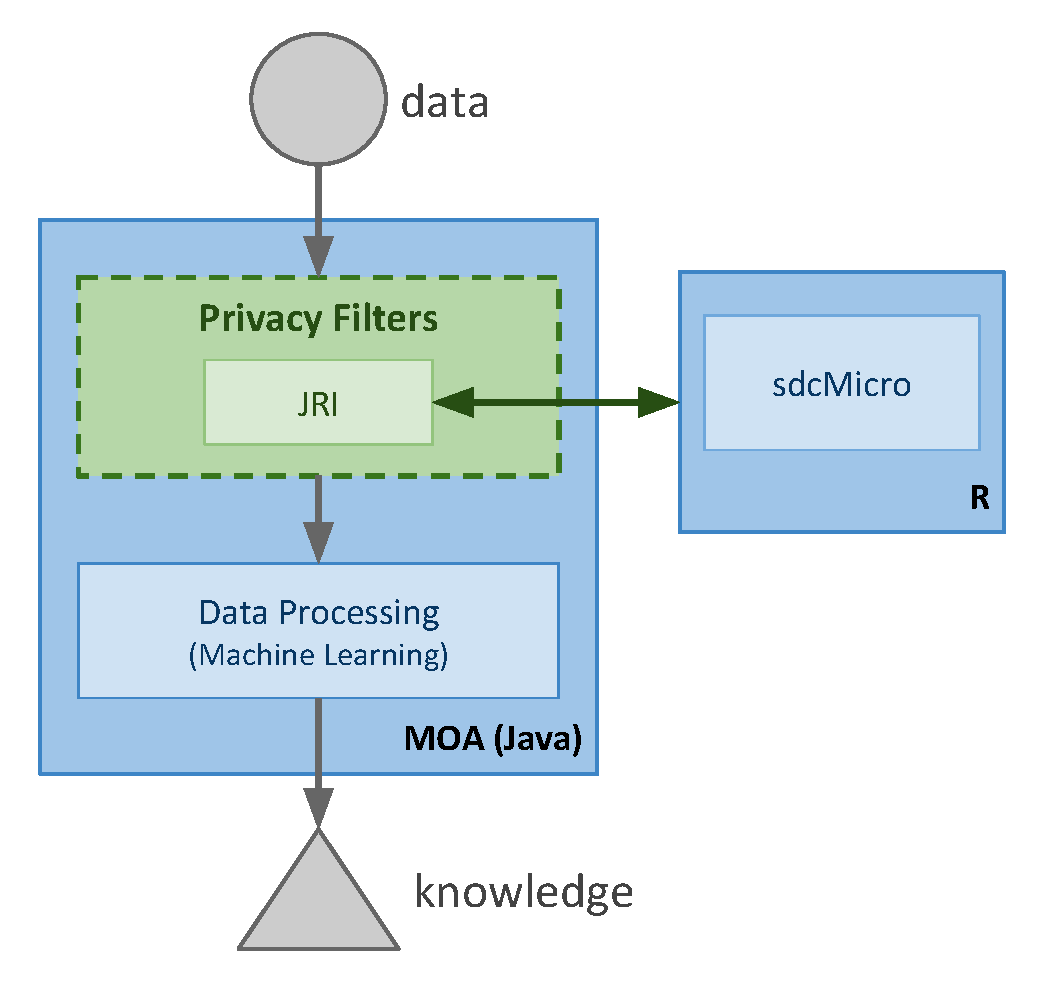
\includegraphics[width=1.0\textwidth]{figures/moa-ppsm-JRI.pdf}
		\caption{Data flow: R/Java hybrid solution.}
		\label{fig:ppsm-JRI}
	\end{minipage}\hfill
	\begin{minipage}[t]{.5\textwidth}
		\centering
		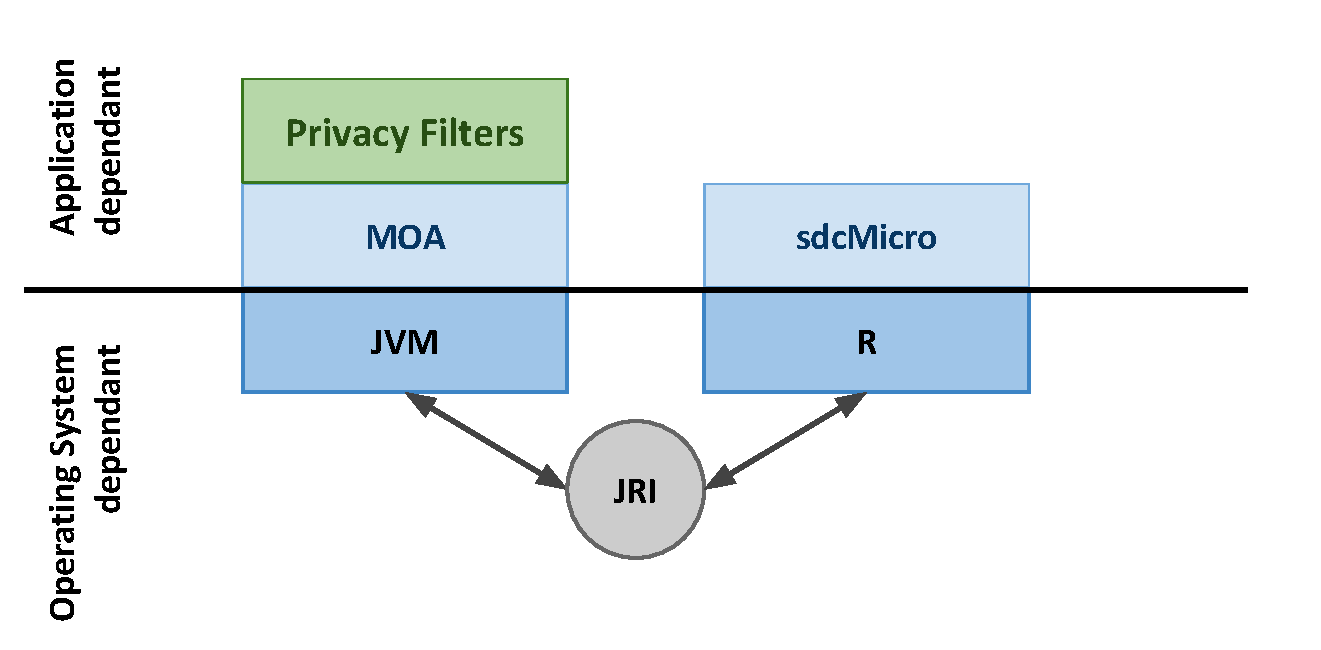
\includegraphics[width=1.2\textwidth]{figures/moa-ppsm-JRI-arch.pdf}
		\caption{Hybrid solution architechture: strong dependencies.}
		\label{fig:ppsm-JRI-arch}
	\end{minipage}
\end{figure}

As can be seen in figures \ref{fig:ppsm-JRI} and \ref{fig:ppsm-JRI-arch}, the \texttt{sdcMicro} library would be used from MOA by developing an adapter (a wrapper) to interconnect the Java and R execution environments. There are some benefits of taking this approach, but also some drawbacks:

\begin{itemize}
	\item \textbf{Faster development:} the only new piece of software to be developed is the wrapper or interconnect between MOA and the \texttt{sdcMicro} package.
	\item BLA BLA
\end{itemize}

\begin{figure}[h]
	\centering
	\begin{minipage}[t]{.45\textwidth}
		\centering
		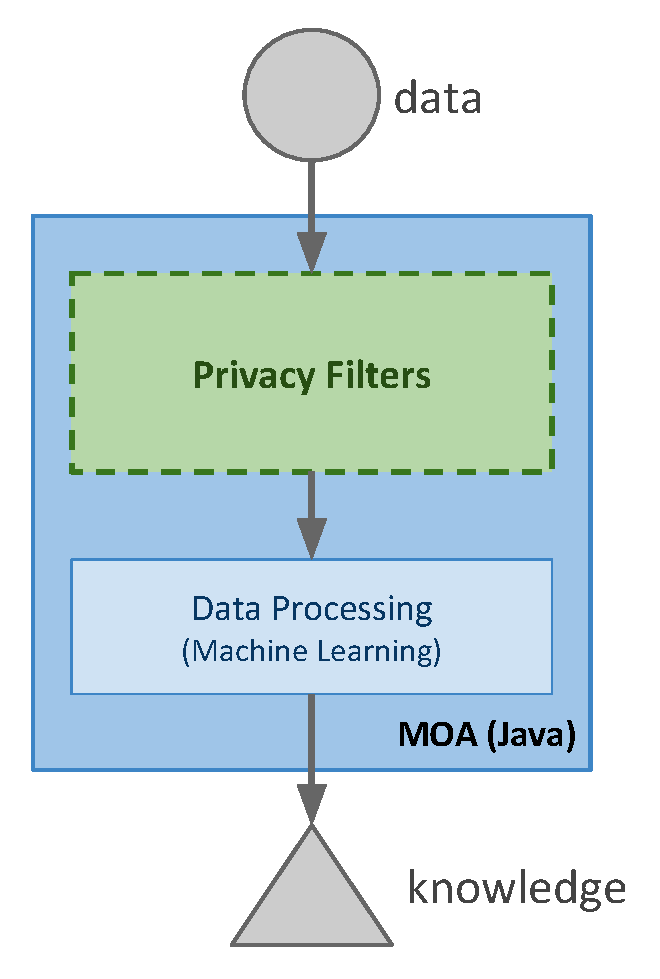
\includegraphics[width=.7\textwidth]{figures/moa-ppsm-JAVA.pdf}
		\caption{Data flow: pure Java solution.}
		\label{fig:ppsm-JAVA}
	\end{minipage}\hfill
	\begin{minipage}[t]{.45\textwidth}
		\centering
		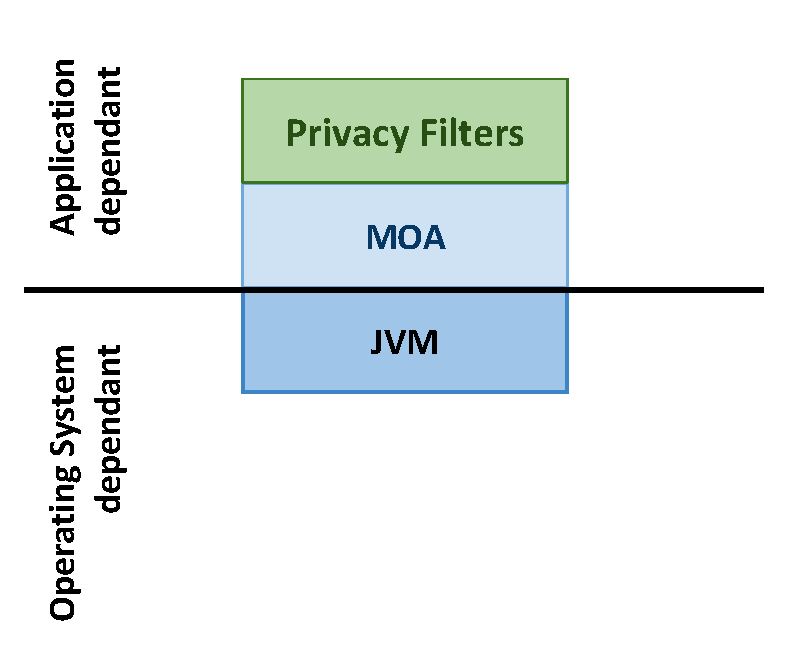
\includegraphics[width=1.0\textwidth]{figures/moa-ppsm-JAVA-arch.pdf}
		\caption{Pure Java solution architechture: few dependencies.}
		\label{fig:ppsm-JAVA-arch}
	\end{minipage}
\end{figure}

\subsection{Implemented algorithms}

\subsection{Roadmap}

\subsubsection{Proposed PPSM methods}

\subsubsection{Results generation}